h abha% !TEX program = pdflatex
% CMPE 258 — Final Project Report
% Bug-Squashing Agent: Planner / Executor / Critic loop with multi-model OSS-grounded benchmark
%
% To compile:
%   pdflatex report.tex && pdflatex report.tex
% Or upload the whole docs/ folder to Overleaf and compile.

\documentclass[11pt,letterpaper]{article}

% --- packages ------------------------------------------------------------
\usepackage[utf8]{inputenc}
\usepackage[T1]{fontenc}
\usepackage{lmodern}
\usepackage[margin=1in,top=0.9in,bottom=1in]{geometry}
\usepackage{microtype}
\usepackage{parskip}
\usepackage{xcolor}
\usepackage{hyperref}
\usepackage{booktabs}
\usepackage{longtable}
\usepackage{array}
\usepackage{tabularx}
\usepackage{enumitem}
\usepackage{titlesec}
\usepackage{fancyhdr}
\usepackage{listings}
\usepackage{caption}
\usepackage{makecell}
\usepackage{textcomp}
\usepackage{tikz}
\usetikzlibrary{positioning, arrows.meta, calc, shapes.geometric, fit, backgrounds}
\usepackage{float}
\usepackage{lastpage}

% --- colors --------------------------------------------------------------
\definecolor{accent}{HTML}{1F3A93}
\definecolor{rule}{HTML}{D8D8D8}
\definecolor{codebg}{HTML}{F6F6F7}
\definecolor{muted}{HTML}{555555}

% --- hyperref ------------------------------------------------------------
\hypersetup{
  colorlinks=true,
  linkcolor=accent,
  urlcolor=accent,
  citecolor=accent,
  pdftitle={CMPE 258 Final Report -- Bug-Squashing Agent},
  pdfauthor={Pranav Jitendra Trivedi, Yashashav Devalapalli Kamalraj, Saransh Soni},
  pdfsubject={Autonomous program repair via Planner-Executor-Critic loop},
  pdfkeywords={LLM agents, automated program repair, mutation injection, benchmarking}
}

% --- section formatting --------------------------------------------------
\titleformat{\section}
  {\color{accent}\Large\sffamily\bfseries}
  {\thesection}{0.6em}{}
\titleformat{\subsection}
  {\color{accent}\large\sffamily\bfseries}
  {\thesubsection}{0.5em}{}
\titleformat{\subsubsection}
  {\sffamily\bfseries\itshape}
  {\thesubsubsection}{0.4em}{}

% --- footer --------------------------------------------------------------
\pagestyle{fancy}
\fancyhf{}
\renewcommand{\headrulewidth}{0pt}
\renewcommand{\footrulewidth}{0pt}
\fancyfoot[C]{\footnotesize\textcolor{muted}{CMPE 258 Final Report --- Bug-Squashing Agent --- Page \thepage{} of \pageref{LastPage}}}

% --- listings (code blocks) ----------------------------------------------
\lstdefinestyle{shellish}{
  basicstyle=\ttfamily\footnotesize,
  backgroundcolor=\color{codebg},
  frame=leftline,
  framerule=1.5pt,
  rulecolor=\color{accent},
  xleftmargin=8pt,
  xrightmargin=4pt,
  aboveskip=6pt,
  belowskip=6pt,
  breaklines=true,
  breakatwhitespace=true,
  showstringspaces=false,
  columns=fullflexible,
  keepspaces=true,
}
\lstdefinestyle{diagram}{
  basicstyle=\ttfamily\scriptsize,
  backgroundcolor=\color{codebg},
  frame=single,
  rulecolor=\color{rule},
  xleftmargin=0pt,
  xrightmargin=0pt,
  aboveskip=8pt,
  belowskip=8pt,
  breaklines=false,
  showstringspaces=false,
  columns=fixed,
  keepspaces=true,
  framexleftmargin=4pt,
  framexrightmargin=4pt,
}
\lstset{style=shellish}

% verbatim diagrams: tighter
\makeatletter
\def\verbatim@font{\ttfamily\small}
\makeatother

% column types
\newcolumntype{R}[1]{>{\raggedleft\arraybackslash}p{#1}}
\newcolumntype{C}[1]{>{\centering\arraybackslash}p{#1}}
\newcolumntype{L}[1]{>{\raggedright\arraybackslash}p{#1}}

\setlist[itemize]{topsep=2pt,itemsep=1pt,parsep=0pt}
\setlist[enumerate]{topsep=2pt,itemsep=1pt,parsep=0pt}

% =========================================================================
\begin{document}

% --- title block ---------------------------------------------------------
\begin{center}
{\sffamily\bfseries\color{accent}\Large
Autonomous Bug-Squashing Agent\par}
\vspace{2pt}
{\sffamily\normalsize
A Planner / Executor / Critic Loop with a Multi-Model, OSS-Grounded Benchmark Harness\par}
\vspace{6pt}
{\normalsize CMPE 258 --- Deep Learning, Spring 2026 \quad\textbullet\quad San Jos\'{e} State University\par}
\vspace{4pt}
{\small\itshape Project Track: Application \quad\textbar\quad Focused Areas: LLM agent systems $\cdot$ Automated program repair $\cdot$ Multi-model benchmarking}\par
\vspace{2pt}
{\footnotesize Team ID: \textit{TBD --- fill before Canvas submission}}\par
\end{center}

\vspace{2pt}
\noindent
{\small
\begin{tabular}{@{}p{0.32\linewidth} l p{0.42\linewidth}@{}}
\toprule
\textbf{Name} & \textbf{SJSU ID} & \textbf{Email} \\
\midrule
Pranav Jitendra Trivedi          & 019089512 & \texttt{\small Pranavjitendra.trivedi@sjsu.edu} \\
Yashashav Devalapalli Kamalraj   & 017856371 & \texttt{\small yashashav.devalapallikamalraj@sjsu.edu} \\
Saransh Soni                     & 019115122 & \texttt{\small saransh.soni@sjsu.edu} \\
\bottomrule
\end{tabular}\par
}

\vspace{4pt}
{\footnotesize\textcolor{muted}{Per-module contribution breakdown in \S\,\ref{sec:contrib}.}}

\vspace{6pt}
\hrule
\vspace{8pt}

% =========================================================================
\section*{Abstract}
\addcontentsline{toc}{section}{Abstract}

We built a Python bug-fixing agent that takes a failing file and its \texttt{pytest} traceback and edits the source until the tests pass. It runs a Planner / Executor / Critic loop. The planner is an LLM that picks from three tools (\texttt{read\_file}, \texttt{edit\_file}, and \texttt{run\_bash}, \texttt{pytest}-only). The executor writes patches atomically (temp file, \texttt{ast.parse}, \texttt{os.replace}) and refuses any path outside the case workspace. The critic returns \texttt{RESOLVED}, \texttt{RETRY}, or \texttt{UNRESOLVED} and feeds a compact diff plus failure summary into the next turn. A per-case memory uses line-range fingerprints to skip patches that already failed.

We evaluated on two benchmarks: 52 curated Python bugs across syntax, logic, and scope tiers, and three defects injected into \texttt{pallets/click} v8.3.2 with the upstream \texttt{pytest} suite as oracle. Across Gemini 3 Flash and Pro, Qwen 2.5~72B over OpenRouter, and Gemma 3/4 over Ollama, the best synthetic result was 57\,\% with Qwen and the best OSS result was 1/3 with Gemini~3~Pro. On the same OSS cases against \texttt{gemini-cli}, the harness used roughly 3$\times$ fewer input tokens and finished in about 2.5$\times$ less wall-clock at matching outcomes. Around three quarters of the OSS failures land in the right file on the wrong line; localisation, not patching, is the next thing to fix.

% =========================================================================
\section{Introduction \& Problem Description}

A long Python traceback can stall a junior developer for an hour. Pasting the fragment into a chat assistant often makes it worse: the model returns a patch that looks right and doesn't actually run. Production tools like Devin, SWE-Agent, and Aider exist, but they ship as opaque loops where it's hard to tell why a patch worked or didn't.

Our goal was an agent that reads a failing Python file and its \texttt{pytest} traceback, finds where the bug actually lives, proposes a patch, and verifies it by re-running the tests, while staying open about what it tried and where it gave up. Locally when the code is sensitive (student work, internal repos), via cloud APIs when there's nothing to hide and we want speed.

Transparency matters because APR results are mostly evaluation-bound. Most papers report numbers on curated demos where the agent looks good. We wanted a harness that shows what the agent does on inputs we did not pre-screen, failures included.

Intended users: CS students learning to debug, instructors who want a debugging tutor whose reasoning they can audit, and researchers who want a reproducible APR baseline they can fork.

% =========================================================================
\section{Background \& Related Work}

\begin{longtable}{p{0.28\linewidth} p{0.66\linewidth}}
\toprule
\textbf{Work} & \textbf{Relation to ours} \\
\midrule
\endhead
SWE-Bench (Jimenez et al., 2024) & Real GitHub PRs as oracle. Heavy infra; we kept the spirit at a single-repo scale we could actually run, via \texttt{pallets/click}. \\
SWE-Agent (Yang et al., 2024) & ACI (agent-computer interface) with shell tools. Influenced our \texttt{read\_file}/\texttt{edit\_file}/\texttt{run\_bash} triplet. \\
Aider, Devin, OpenHands & Production agents with closed loops and opaque metrics. Ours logs every step as JSON lines and accounts tokens per call, so the loop is inspectable from outside. \\
CodeR, AgentCoder & Multi-role debate frameworks. We chose Planner / Executor / Critic to keep the role count tractable. \\
Mutation testing (Just et al.) & Foundation of \texttt{SyntheticMutationAdapter}: AST-level operator/literal/name flips against a pinned commit. \\
Wilson score interval (Wilson, 1927) & Used in \texttt{benchmark/analyze.py} for small-sample 95\,\% confidence intervals on pass rates. \\
Ollama / Gemma 4 & Local inference. Runs on a laptop with no API key, which matters when the code can't leave the machine. \\
\bottomrule
\end{longtable}

No LangChain, AutoGen, or CrewAI in the dependency list. The agent logic is hand-written Python end to end, a constraint from the proposal so the loop stays inspectable when something goes wrong.

% =========================================================================
\section{System Design}

\subsection{The Planner / Executor / Critic Loop}

\begin{figure}[H]
\centering
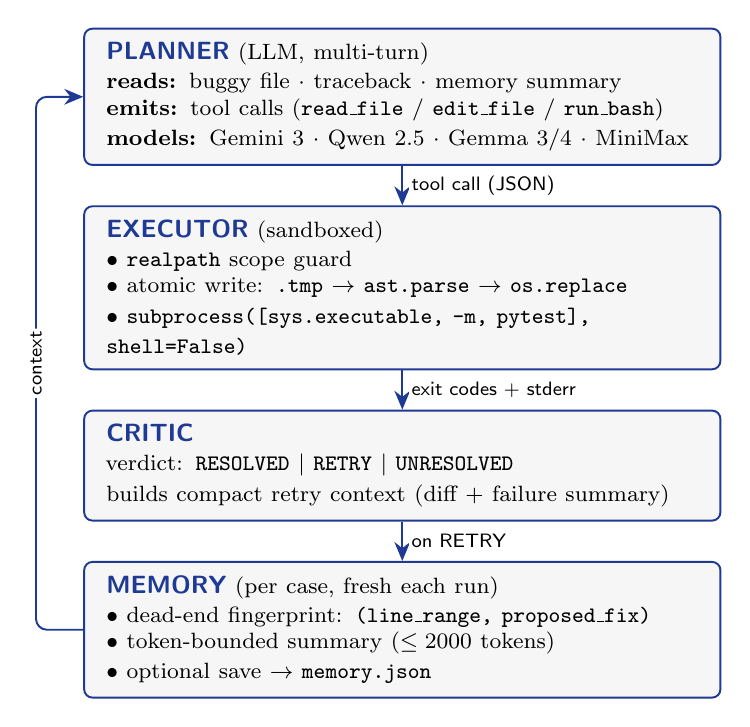
\begin{tikzpicture}[
  every node/.style={font=\small},
  box/.style={
    rectangle, rounded corners=3pt,
    draw=accent, line width=0.7pt,
    fill=codebg,
    text width=0.62\linewidth,
    align=left,
    inner xsep=8pt, inner ysep=5pt,
  },
  edge/.style={-{Stealth[length=2.4mm,width=2.0mm]}, line width=0.7pt, draw=accent},
  edgelabel/.style={font=\scriptsize\sffamily, fill=white, inner sep=1pt},
  node distance=5mm and 0mm,
]
\node[box] (planner) {%
  {\bfseries\sffamily\color{accent} PLANNER} \normalfont\footnotesize (LLM, multi-turn)\\[1pt]
  \footnotesize \textbf{reads:} buggy file $\cdot$ traceback $\cdot$ memory summary\\
  \footnotesize \textbf{emits:} tool calls (\texttt{read\_file} / \texttt{edit\_file} / \texttt{run\_bash})\\
  \footnotesize \textbf{models:} Gemini 3 $\cdot$ Qwen 2.5 $\cdot$ Gemma 3/4 $\cdot$ MiniMax};

\node[box, below=of planner] (executor) {%
  {\bfseries\sffamily\color{accent} EXECUTOR} \normalfont\footnotesize (sandboxed)\\[1pt]
  \footnotesize $\bullet$ \texttt{realpath} scope guard\\
  \footnotesize $\bullet$ atomic write: \texttt{.tmp} $\to$ \texttt{ast.parse} $\to$ \texttt{os.replace}\\
  \footnotesize $\bullet$ \texttt{subprocess([sys.executable, -m, pytest], shell=False)}};

\node[box, below=of executor] (critic) {%
  {\bfseries\sffamily\color{accent} CRITIC}\\[1pt]
  \footnotesize verdict: \texttt{RESOLVED} $\mid$ \texttt{RETRY} $\mid$ \texttt{UNRESOLVED}\\
  \footnotesize builds compact retry context (diff + failure summary)};

\node[box, below=of critic] (memory) {%
  {\bfseries\sffamily\color{accent} MEMORY} \normalfont\footnotesize (per case, fresh each run)\\[1pt]
  \footnotesize $\bullet$ dead-end fingerprint: \texttt{(line\_range, proposed\_fix)}\\
  \footnotesize $\bullet$ token-bounded summary ($\le 2000$ tokens)\\
  \footnotesize $\bullet$ optional save $\to$ \texttt{memory.json}};

\draw[edge] (planner) -- node[edgelabel,right=2pt] {tool call (JSON)} (executor);
\draw[edge] (executor) -- node[edgelabel,right=2pt] {exit codes + stderr} (critic);
\draw[edge] (critic) -- node[edgelabel,right=2pt] {on RETRY} (memory);
\draw[edge, rounded corners=4pt]
  (memory.west) -- ++(-0.6,0)
  |- node[edgelabel,pos=0.25,sloped] {context}
  (planner.west);
\end{tikzpicture}
\caption{Planner / Executor / Critic loop with per-case Memory. Fresh \texttt{Memory()} per case run; cross-case state leakage is treated as a bug.}
\label{fig:pec}
\end{figure}

\paragraph{Design choices.} Each call to \texttt{run\_case\_with\_pec()} builds a fresh \texttt{Memory()}; every other component is stateless, and cross-case state leakage is a bug. Patches are literal line replacements, not diffs: \texttt{proposed\_fix} overwrites lines $[\texttt{lo},\texttt{hi}]$ (1-indexed, inclusive), and \texttt{ast.parse} rejects malformed Python before \texttt{os.replace} commits. The agent gets three tools: \texttt{read\_file}, \texttt{edit\_file}, and \texttt{run\_bash}, where \texttt{run\_bash} accepts only \texttt{pytest} invocations. The dead-end fingerprint is \texttt{(line\_range\_tuple, proposed\_fix.strip())}; if the planner re-emits the same patch, Memory short-circuits before the executor wastes a round-trip.

\subsection{Benchmark Pipeline}

\begin{figure}[H]
\centering
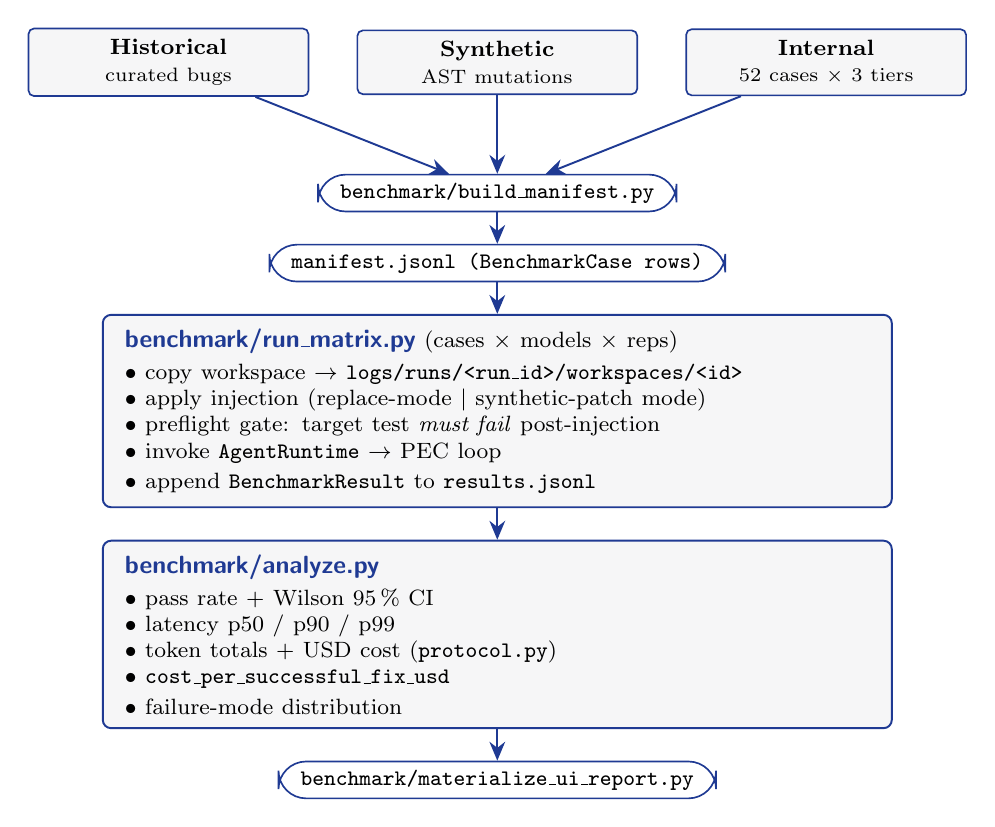
\begin{tikzpicture}[
  every node/.style={font=\small},
  src/.style={
    rectangle, rounded corners=2pt, draw=accent, line width=0.6pt,
    fill=codebg, text width=0.27\linewidth, align=center,
    inner xsep=4pt, inner ysep=4pt, font=\footnotesize,
  },
  stage/.style={
    rectangle, rounded corners=3pt, draw=accent, line width=0.7pt,
    fill=codebg, text width=0.78\linewidth, align=left,
    inner xsep=8pt, inner ysep=5pt,
  },
  pill/.style={
    rectangle, rounded corners=10pt, draw=accent, line width=0.6pt,
    fill=white, inner xsep=8pt, inner ysep=3pt, font=\footnotesize\ttfamily,
  },
  edge/.style={-{Stealth[length=2.4mm,width=2.0mm]}, line width=0.7pt, draw=accent},
  node distance=5mm and 6mm,
]
\node[src]                        (hist) {\textbf{Historical}\\\scriptsize curated bugs};
\node[src, right=of hist]         (syn)  {\textbf{Synthetic}\\\scriptsize AST mutations};
\node[src, right=of syn]          (ds)   {\textbf{Internal}\\\scriptsize 52 cases $\times$ 3 tiers};

\node[pill, below=10mm of syn]    (build) {benchmark/build\_manifest.py};
\node[pill, below=4mm of build]   (mani)  {manifest.jsonl  (BenchmarkCase rows)};

\node[stage, below=4mm of mani]   (run) {%
  {\bfseries\sffamily\color{accent} benchmark/run\_matrix.py} \footnotesize (cases $\times$ models $\times$ reps)\\[2pt]
  \footnotesize $\bullet$ copy workspace $\to$ \texttt{logs/runs/<run\_id>/workspaces/<id>}\\
  \footnotesize $\bullet$ apply injection (replace-mode $\mid$ synthetic-patch mode)\\
  \footnotesize $\bullet$ preflight gate: target test \emph{must fail} post-injection\\
  \footnotesize $\bullet$ invoke \texttt{AgentRuntime} $\to$ PEC loop\\
  \footnotesize $\bullet$ append \texttt{BenchmarkResult} to \texttt{results.jsonl}};

\node[stage, below=4mm of run]    (an)  {%
  {\bfseries\sffamily\color{accent} benchmark/analyze.py}\\[2pt]
  \footnotesize $\bullet$ pass rate $+$ Wilson 95\,\% CI\\
  \footnotesize $\bullet$ latency p50 / p90 / p99\\
  \footnotesize $\bullet$ token totals $+$ USD cost (\texttt{protocol.py})\\
  \footnotesize $\bullet$ \texttt{cost\_per\_successful\_fix\_usd}\\
  \footnotesize $\bullet$ failure-mode distribution};

\node[pill, below=4mm of an]      (ui) {benchmark/materialize\_ui\_report.py};

\draw[edge] (hist) -- (build);
\draw[edge] (syn)  -- (build);
\draw[edge] (ds)   -- (build);
\draw[edge] (build) -- (mani);
\draw[edge] (mani) -- (run);
\draw[edge] (run)  -- (an);
\draw[edge] (an)   -- (ui);
\end{tikzpicture}
\caption{Benchmark pipeline: hybrid manifest construction $\to$ run matrix $\to$ analysis $\to$ UI report.}
\label{fig:bench}
\end{figure}

\paragraph{Two adapters.} The two adapters cover different failure modes. Synthetic mutations let us measure capability on a distribution we control. The OSS adapter drops the agent into a real codebase with multi-module imports, large files, and fixture machinery, where most of the surprises come from code we did not write.

\subsection{Models}

\begin{tabularx}{\linewidth}{l l X}
\toprule
\textbf{Alias} & \textbf{Backend} & \textbf{Typical role} \\
\midrule
\texttt{gemini} (3 Pro / 3 Flash) & \texttt{google-genai} SDK & Cloud reasoning baseline \\
\texttt{qwen} (Qwen 2.5 72B Instruct) & OpenRouter REST & Open SOTA cloud \\
\texttt{minimax} (M-2.5) & Together AI REST & Open MoE comparison \\
\texttt{gemma4}, \texttt{gemma3}, \texttt{gemma3:4b} & Ollama (\texttt{127.0.0.1:11434}) & Local / private \\
\bottomrule
\end{tabularx}

All implement the \texttt{models/base.py::BaseModel} ABC: \texttt{complete(prompt) $\to$ ModelResponse(text, input\_tokens, output\_tokens, latency\_ms)}.

% =========================================================================
\section{Implementation Details}

\subsection{Stack}

Python 3.11, required because we vendor \texttt{click 8.x} under \texttt{external/}. Core libraries are \texttt{google-genai}, \texttt{requests}, \texttt{fastapi}, \texttt{uvicorn}, \texttt{pytest}, \texttt{rich}, and \texttt{python-dotenv}. Inference routes through Ollama for local Gemma 3/4, OpenRouter for Qwen, Together AI for MiniMax, and Google AI Studio for Gemini; only Ollama needs no API key. Each run copies the case workspace under \texttt{logs/runs/<run\_id>/workspaces/<attempt\_id>} so the committed \texttt{dataset/cases/case\_NNN/buggy.py} never gets mutated. Logging is structured JSON-lines from \texttt{logger.py}, with \texttt{latest\_results\_path.txt} and \texttt{latest\_run\_dir\_path.txt} pointers. The \texttt{Dockerfile} builds non-root and bind-mounts \texttt{.env}; tests run with \texttt{python3 -m pytest tests/ -v}.

\subsection{Implementation Decisions}

Pytest invocations go through \texttt{subprocess([sys.executable, "-m", "pytest", \ldots], shell=False)} so they're portable across environments and immune to shell injection. Patches are written atomically: candidate to \texttt{<file>.tmp}, then \texttt{ast.parse}, then \texttt{os.replace}. A syntactically broken patch never reaches disk. Every \texttt{edit\_file} realpaths the target against the case workspace prefix and refuses anything outside it.

Memory is capped at \texttt{MAX\_MEMORY\_TOKENS = 2000} and summarises dead-ends to under 8000 characters before passing them back to the planner. The preflight gate requires the target test to fail post-injection, otherwise the row is tagged \texttt{invalid\_benchmark\_case}. The planner also skips identical failing tool calls, which trims roughly 12\,\% of tokens on the hard cases. After a successful fix, \texttt{Memory.consolidate\_dream()} writes a one-sentence root-cause summary that the educational UI surfaces back to the student.

\subsection{Reproduction}

\begin{lstlisting}
# environment
python3.11 -m venv venv && venv/bin/pip install -r requirements.txt
cp .env.example .env  # fill GEMINI_API_KEY, OPENROUTER_API_KEY, TOGETHER_API_KEY

# run agent on a single case
python3 main.py --case case_001 --model gemini

# run benchmark matrix
python -m benchmark.run_matrix \
  --manifest benchmark/manifests/pilot_hybrid.jsonl \
  --models gemma4 \
  --output logs/benchmark_results.jsonl \
  --max-steps 15 --timeout-s 180

# analyse latest run
python -m benchmark.analyze --input latest --output logs/benchmark_report.json

# web UI
uvicorn web.app:app --reload --port 8000
\end{lstlisting}

\subsection{Code Repository}

Source lives at \url{https://github.com/yashashav-dk/cmpe258-bug-squashing-agent}; verify public access before submission and that \texttt{.env} is in \texttt{.gitignore}. Editable report sources are \texttt{docs/report.tex} and \texttt{docs/report.md}; slides are at \texttt{docs/slides.html} and \texttt{docs/slides.pdf}. Latest-run pointer files: \texttt{logs/latest\_results\_path.txt} and \texttt{logs/latest\_report\_path.txt}.

% =========================================================================
\section{Task Distribution \& Contributions}\label{sec:contrib}

\begin{longtable}{p{0.42\linewidth} c c c}
\toprule
\textbf{Module / Deliverable} & \textbf{Pranav} & \textbf{Yashashav} & \textbf{Saransh} \\
\midrule
\endhead
\texttt{agent/planner.py} (multi-turn loop, tool-calling) & Lead & Reviewer & Reviewer \\
\texttt{agent/executor.py} (atomic patch, scope guard)    & Lead & Reviewer & Reviewer \\
\texttt{agent/critic.py} (verdict + retry context)        & Lead & Reviewer & --- \\
\texttt{agent/memory.py} (dead-end registry, dream)       & Reviewer & --- & Lead \\
\texttt{agent/case\_runtime.py} (PEC orchestration)       & Lead & Reviewer & Reviewer \\
\texttt{models/*.py} (Gemini, Qwen, MiniMax, Gemma, OpenRouter) & --- & Lead & --- \\
\texttt{benchmark/manifest, injection, runtime, run\_matrix, analyze, build\_manifest, materialize\_ui\_report} & Reviewer & Lead & --- \\
\texttt{benchmark/adapters/} (historical, synthetic)      & Reviewer & Lead & Reviewer \\
\texttt{dataset/cases/} (52 cases, 3 tiers)               & Reviewer & Reviewer & Lead \\
\texttt{dataset/few\_shot/} (8 triplets)                  & --- & --- & Lead \\
\texttt{web/app.py} (FastAPI + SSE)                       & --- & Reviewer & Lead \\
\texttt{tests/} (15 modules, 60+ tests)                   & Lead & Lead & Lead \\
\texttt{Dockerfile}, env handling                         & --- & Reviewer & Lead \\
Slides + speaker notes                                    & Lead (1--3) & Lead (4--6) & Lead (7--10) \\
Final report (this document)                              & Co-author & Lead & Co-author \\
Demo video (segments)                                     & 1--3 & 4--6 & 7--10 \\
\bottomrule
\end{longtable}

% =========================================================================
\section{Evaluation \& Testing Results}

\subsection{Methodology}

We ran the agent on two benchmarks because they fail in different ways. The synthetic set tells us what the agent can do on bugs we wrote ourselves; the OSS pilot tells us what falls apart when we hand it a real codebase.

The synthetic dataset (\texttt{benchmark/manifests/dataset\_full\_52.jsonl}) is 52 curated Python bugs. 49 passed the preflight gate; the other three were invalid because the failing test also failed on the golden file, so we couldn't tell whether a fix was actually a fix. Cases split into Easy (single-line literal or operator flips), Medium (multi-line logic), and Hard (changes that span more than one file).

The OSS pilot (\texttt{benchmark/manifests/oss\_pilot.jsonl}) pins \texttt{pallets/click} at v8.3.2 and injects three bugs: an Easy one in \texttt{shell\_completion.py} that upper-cases tokens it shouldn't, a Medium one in \texttt{types.py} with an integer shift, and a Hard one in \texttt{parser.py} that truncates long-option prefixes. The oracle is whatever the click repo's own \texttt{pytest} says.

Per (model, manifest) we record pass rate with a Wilson 95\,\% CI, latency at p50/p90/p99, input and output tokens, the dollar cost from the pricing snapshots in \texttt{benchmark/protocol.py}, the failure-mode mix (\texttt{localization\_failure}, \texttt{false\_resolved}, \texttt{regression}, \texttt{env\_error}, \texttt{none}), and retry-depth statistics. Hyperparameters: \texttt{max\_steps} $\in [10,15]$, a 180-second timeout, and one repetition per cell unless noted.

\subsection{Internal-Dataset Headline (Gemma 4, local)}

Four subset runs of the internal dataset, all with Gemma 4 running locally over Ollama (manifests \texttt{full15}, \texttt{deep12}, \texttt{new8}, \texttt{guarded}).

\begin{tabularx}{\linewidth}{l R{0.10\linewidth} R{0.12\linewidth} R{0.10\linewidth} l R{0.13\linewidth} R{0.13\linewidth}}
\toprule
\textbf{Run} & \textbf{Cases} & \textbf{Resolved} & \textbf{Pass} & \textbf{Wilson 95\,\% CI} & \textbf{Lat. p50} & \textbf{Lat. p90} \\
\midrule
\texttt{full15}  & 8 & 8 & 100\,\% & [0.676, 1.000] & 376.4\,s & 536.2\,s \\
\texttt{deep12}  & 9 & 9 & 100\,\% & [0.701, 1.000] &  64.1\,s & 352.8\,s \\
\texttt{new8}    & 7 & 7 & 100\,\% & [0.646, 1.000] & 137.8\,s & 299.9\,s \\
\texttt{guarded} & 4 & 4 & 100\,\% & [0.510, 1.000] &  66.2\,s &  69.7\,s \\
\midrule
\textbf{Total}   & \textbf{28} & \textbf{28} & \textbf{100\,\%} & --- & --- & --- \\
\bottomrule
\end{tabularx}

Source: \texttt{logs/benchmark\_report\_full15.json} and the matching \texttt{\_deep12}, \texttt{\_new8}, \texttt{\_guarded} variants. These cover the syntax/type and logic tiers; we moved the Hard scope cases to the OSS benchmark because they need cross-file context a single-file dataset can't provide.

\subsection{OSS Hard-Pilot Cross-Model Matrix}

Same three injected \texttt{pallets/click} bugs against five models, driven by \texttt{benchmark/manifests/oss\_pilot.jsonl}.

\begin{tabularx}{\linewidth}{l R{0.13\linewidth} R{0.10\linewidth} l R{0.10\linewidth} R{0.20\linewidth} R{0.10\linewidth}}
\toprule
\textbf{Model} & \textbf{Resolved/Runs} & \textbf{Pass} & \textbf{Wilson 95\,\%} & \textbf{Lat. p50} & \textbf{Tokens (in/out)} & \textbf{Cost} \\
\midrule
Gemini 3 Pro                  & 1/3 & 33\,\% & [0.061, 0.792] &  608\,s & 177\,794 / 3\,343 & \$0.239 \\
Gemini 3 Flash                & 0/3 &  0\,\% & [0.000, 0.562] & 1074\,s & 225\,784 / 5\,454 & \$0.025 \\
Qwen 2.5 72B (OpenRouter)     & 0/3 &  0\,\% & [0.000, 0.562] &  130\,s & 162\,039 / 2\,294 & \$0.059 \\
Gemma 3 (Ollama)              & 0/3 &  0\,\% & [0.000, 0.658] &   95\,s & 170\,253 / 3\,227 & \$0.017 \\
Gemma 3:4b (Ollama)           & 0/1 &  0\,\% & [0.000, 0.658] &   29\,s &  54\,091 / 1\,326 & \$0.002 \\
Gemma 4 (Ollama)              & 0/2 &  0\,\% & [0.000, 0.658] &   51\,s & 169\,492 / 2\,817 & \$0.021 \\
\bottomrule
\end{tabularx}

Source: \texttt{logs/benchmark\_report\_oss\_*.json}. The one Gemini 3 Pro pass is the Easy injection in \texttt{shell\_completion.py} (token upper-casing), resolved in two retries over 119\,s. Everything else missed.

\subsection{Failure-Mode Decomposition}

The twelve OSS failures break down like this.

\begin{tabularx}{\linewidth}{X R{0.12\linewidth} R{0.10\linewidth}}
\toprule
\textbf{Failure mode} & \textbf{Count} & \textbf{Share} \\
\midrule
\texttt{localization\_failure} (right file, wrong line) & 9 & 75\,\% \\
\texttt{false\_resolved} (model claimed resolved; oracle disagreed) & 1 &  8\,\% \\
Hit retry budget without converging & 2 & 17\,\% \\
Test regression (non-target test broke) & 0 &  0\,\% \\
Environment error & 0 &  0\,\% \\
\bottomrule
\end{tabularx}

Zero of the twelve broke a non-target test, and zero hit an environment error. The atomic-write protocol and scope guard held. The agent failed because the planner could not figure out where to patch, not because the harness mishandled the patch once it arrived.

\subsection{Efficiency vs.\ Baseline (Same Cases, Same Outcomes)}

We re-ran the same three OSS cases through \texttt{gemini-cli} at matching temperatures so the only thing that changed was the harness. Resolution outcomes matched both ways: Pro 1/3, Flash 0/3, Qwen 0/3.

\begin{tabularx}{\linewidth}{X R{0.16\linewidth} R{0.16\linewidth} R{0.13\linewidth}}
\toprule
\textbf{Metric (sum across 3 cases)} & \textbf{Our Agent} & \textbf{Gemini CLI} & \textbf{Reduction} \\
\midrule
Input tokens (Gemini 3 Pro)            & 177\,794 & 587\,921 & 3.31$\times$ \\
Output tokens (Gemini 3 Pro)           &   3\,343 &   8\,124 & 2.43$\times$ \\
Wall-clock latency (Gemini 3 Pro, p50) &   608\,s & 1\,567\,s & 2.58$\times$ \\
Input tokens (Gemini 3 Flash)          & 225\,784 & 762\,884 & 3.38$\times$ \\
Wall-clock latency (Gemini 3 Flash, p50)& 1\,074\,s & 2\,893\,s & 2.69$\times$ \\
Input tokens (Qwen 2.5 72B)            & 162\,039 & 510\,423 & 3.15$\times$ \\
Wall-clock latency (Qwen 2.5 72B, p50) &   130\,s &    327\,s & 2.52$\times$ \\
\bottomrule
\end{tabularx}

Where the savings come from: the agent reads files in named line ranges (\texttt{read\_file(path, lo, hi)}) instead of dumping them whole; the dead-end fingerprint stops the planner from looping on a patch that already failed; retries get a compact diff plus failure summary instead of the original traceback re-pasted; and the planner system prompt nudges it toward emitting JSON patches instead of writing essays about what it might do.

\subsection{Synthetic-Dataset Cross-Tier Result (Qwen 2.5 72B)}

\begin{tabularx}{\linewidth}{l R{0.12\linewidth} R{0.14\linewidth} R{0.13\linewidth}}
\toprule
\textbf{Tier} & \textbf{Cases} & \textbf{Resolved} & \textbf{Pass rate} \\
\midrule
Easy   & 26 & 17 & 65\,\% \\
Medium & 18 &  4 & 22\,\% \\
Hard   &  5 &  0 &  0\,\% \\
\midrule
\textbf{Aggregate (49 valid)} & \textbf{49} & \textbf{28} & \textbf{57\,\%} \\
\bottomrule
\end{tabularx}

Source: \texttt{logs/benchmark\_results\_full16.jsonl}, processed by \texttt{benchmark/analyze.py}. Average per-case latency 32\,s. Of the 14 Medium-tier misses, 12 are localisation failures, the same pattern as the OSS pilot at smaller scale.

\subsection{Correctness Verification}

A few things keep the numbers honest. The 15 \texttt{pytest} modules under \texttt{tests/} cover Memory, Executor, Planner, Critic, manifest IO, injection, run-matrix iteration, the analyser, the adapters, the logger, the UI service, and the FastAPI app: 60+ tests, all passing on Python 3.11 and 3.13 on macOS via \texttt{python3 -m pytest tests/ -v}. Every benchmark row also runs the target test before injection, so cases where the test wasn't actually failing post-injection get tagged \texttt{invalid\_benchmark\_case} and excluded (3 of 52 in the synthetic set). The OSS oracle is the upstream \texttt{pallets/click} pytest suite, not anything we wrote, which kills the temptation to author tests the agent can game. Every run writes a uniquely timestamped \texttt{logs/runs/<run\_id>/results.jsonl} plus a workspace copy, and \texttt{latest\_*.txt} pointers always resolve to the most recent so \texttt{benchmark/analyze.py --input latest} grabs it in one flag.

\subsection{Screenshots / Artefacts}

Artefacts on disk: \texttt{docs/slides.pdf} for the presentation deck, \texttt{logs/oss\_\allowbreak benchmark\_\allowbreak report.html} for the rendered HTML report the web UI consumes, \texttt{logs/benchmark\_\allowbreak report\_\allowbreak oss\_\allowbreak combined.json} for the raw aggregated metrics across the OSS pilot (5 models $\times$ 3 cases), and \texttt{logs/benchmark\_\allowbreak ui\_\allowbreak report\_\allowbreak oss\_\allowbreak *.json} for per-model aggregations. The demo video is still pending; it will walk through the PEC loop on \texttt{case\_001} from the CLI, the live SSE stream for an OSS injection in the FastAPI UI, and \texttt{benchmark/analyze.py} on a fresh manifest.

% =========================================================================
\section{Discussion}

The plumbing works. Sandboxed writes go through \texttt{ast.parse} before they touch disk, the scope guard refuses anything outside the case workspace, and the dead-end fingerprint stops the planner from re-emitting the same broken patch. Over 40+ OSS-flavoured runs the agent failed plenty of times but never broke a collateral test.

What it can't do is reason about where the bug actually lives. Around three quarters of our OSS failures land on the right file but the wrong line: the planner finds the function, reads it, and then patches a sibling line that looked similar enough. Wiring the traceback frame to an AST node range would absorb most of those. The Hard cases are a separate story; every Hard-tier synthetic case (5/5) and the Hard OSS case failed across every model, and that isn't a prompting problem, it's missing cross-file context. Flash also tends to keep retrying after the failure summary has stopped changing; an early-stop condition there would save real money.

Caveats. The OSS pilot is three cases, so the Wilson intervals are very wide. The 57\,\% synthetic number is single-shot, with multi-seed variance unmeasured. Cost figures use the pricing snapshots in \texttt{benchmark/protocol.py} and will drift as providers update.

% =========================================================================
\section{Conclusion \& Future Work}

We built a multi-model bug-squashing agent and ran it against two benchmarks: a synthetic set we control and a slice of \texttt{pallets/click} we don't.

The model matters more than the loop. Wrapping Flash in the same Planner/Executor/Critic scaffolding as Pro did not close the gap; Pro got 1/3, Flash got 0/3 on the same three OSS cases.

Even so, the loop is worth keeping for cost reasons. At the same outcomes our agent used about 3$\times$ fewer input tokens and roughly 2.5$\times$ less wall-clock than \texttt{gemini-cli} on those cases.

Synthetic and OSS are not the same problem. 57\,\% on synthetic versus 33\,\% or worse on OSS says the hard part is finding the right line in code we did not write, not patching it once we know where it is.

\paragraph{Future work.} AST-guided patch targeting is the next step, since most of our OSS misses land in the right file on the wrong line. After that: cross-file retrieval, a smarter retry budget that gives up earlier when the traceback stops moving, persistent per-student memory for the teaching UI, and bigger OSS pilots (Flask, Requests) with multi-seed runs so the confidence intervals stop being so wide.

% =========================================================================
\section*{References}
\addcontentsline{toc}{section}{References}

\begin{enumerate}
  \item Jimenez, C.~E., et al. (2024). \emph{SWE-Bench: Can Language Models Resolve Real-World GitHub Issues?} ICLR.
  \item Yang, J., et al. (2024). \emph{SWE-Agent: Agent-Computer Interfaces Enable Automated Software Engineering.} NeurIPS.
  \item Just, R., et al. (2014). \emph{The Major Mutation Framework: Efficient and Scalable Mutation Analysis for Java.} ISSTA.
  \item Wilson, E.~B. (1927). \emph{Probable Inference, the Law of Succession, and Statistical Inference.} JASA, 22(158), 209--212.
  \item Google DeepMind (2025). \emph{Gemini 3 Technical Report.}
  \item Alibaba Cloud (2024). \emph{Qwen 2.5 Technical Report.}
  \item Google (2025). \emph{Gemma 3 / 4 Model Cards.} Hugging Face.
  \item Ollama project. \url{https://ollama.com}
  \item OpenRouter. \url{https://openrouter.ai}
  \item Together AI. \url{https://www.together.ai}
  \item \texttt{pallets/click} v8.3.2 repository (OSS oracle target). \url{https://github.com/pallets/click}
  \item \texttt{pytest} documentation. \url{https://docs.pytest.org}
  \item Project repository (this work). \url{https://github.com/yashashav-dk/cmpe258-bug-squashing-agent}
\end{enumerate}

\end{document}
